\section{Assignment}

\subsection{Q-1: Boston Housing}

\subsubsection*{(a) Explore the Boston dataset in MASS library}
\label{ref:logistic_regression}
The Boston data frame has 506 rows and 14 columns. The data set contains different properties about suburbs of Boston. The types of data are integers and numerics. From the summary of the data frame, the crime median is computed as 0.2561. 

\begin{figure}[H]
\centering
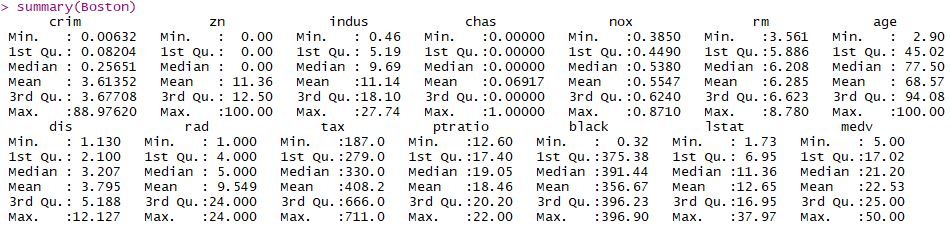
\includegraphics[scale=0.49]{Graphics/Assignment1/ExploreBoston.JPG}
\caption{Descriptive overview of Boston dataset}
\label{fig:logistic_regression_confusions_matrix_001}
\end{figure}


\subsubsection*{(b) Fit classification models}
\textbf{Logistic regression}

\iffalse
Step 1: Load data and run numerical and graphical summaries\\
Step 2: Split the data into training and testing data \\
Step 3: Fit a logistic regression model using training data\\
Step 4: Use the fitted model to do prediction for the test data\\
Step 5: Create the confusion matrix and compute the misclassification rate\\ \\
\fi


In figure \ref{fig:task_1_binomial_logistic_model} the binomial logistic model is explored. The algorithm outputs significant codes which results in the variables with lowest p-values. The p-value expresses whether the null hypothesis should be accepted or rejected. If the p-value is less or equal to the significance level, there is strong evidence to reject the null hypothesis and accept the alternative hypothesis, $H_A$.   
In this case, the hypothesis expresses the influence of the predictor variables to the predicted feature, which is the 'iscrime'. 

The $H_0$ states that a specific predictor variable does not have a strong association to the predicted variable. To find the variables with importance to the predicted value, the null hypothesis has to be rejected, hence using the p-value.    


\begin{figure}[h]
\centering
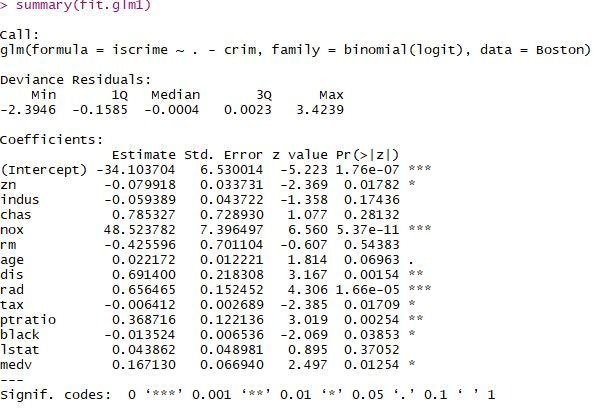
\includegraphics[scale=0.6]{Graphics/Assignment1/LogisticRegressionCoefficientsExplore.JPG}
\caption{Binomial logistic model}
\label{fig:task_1_binomial_logistic_model}
\end{figure}

From figure \ref{fig:task_1_binomial_logistic_model}, the following variables which have a strong influence to the predicted value are: zn, nox, dis, rad, tax, ptratio, black and medv. In this experiment, other subsets of variables will be used with different significance level, shown on table \ref{table_subsets}.

\begin{table}[H]
\centering
\begin{tabular}{|c|c|}
\hline
Sign. Level & Variables                                     \\ \hline
5\%          & zn, nox, dis, rad, tax, ptratio, black, medv \\ \hline
1\%          & nox, dis, rad, ptratio                       \\ \hline
0.1\%        & nox, rad                                     \\ \hline
\end{tabular}
\caption{Subsets in relation to sign. level}
\label{table_subsets}
\end{table}

The misclassification of the models are computed with respect to the different subsets and their variables with the training data as data input. Each model results in a confusion matrix. From the confusion matrix, the misclassification rate and accuracy is computed by using formula from figure \ref{fig:confusion_Matrix} in appendix \ref{app:boston_housing}. The predict function computes the predicted probabilities for crime based on the test data. The predicted probabilities are used to compute if the crime rate is above or below the median. Figure \ref{fig:logistic_regression_confusions_matrix_005}, \ref{fig:logistic_regression_confusions_matrix_001} and \ref{fig:logistic_regression_confusions_matrix_0001} shows the different confusion matrices and error rates for each model with respect to their significance level.  \\

\begin{figure}[H]
\centering
\begin{minipage}{0.32\textwidth}
\centering
    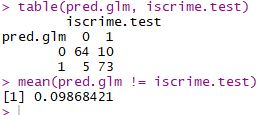
\includegraphics[width=\linewidth, height= 60pt]{Graphics/Assignment1/LogisticRegressionConfusionsMatrix.JPG}
    \caption{Confusion Matrix - sign. level of 0.05}
    \label{fig:logistic_regression_confusions_matrix_005}
\end{minipage}\hfill
\begin{minipage}{0.32\textwidth}
\centering

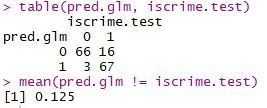
\includegraphics[width=\linewidth, height= 60pt]{Graphics/Assignment1/LogisticRegressionConfusionsMatrix_001.JPG}
    \caption{Confusion Matrix - sign. level of 0.01}
    \label{fig:logistic_regression_confusions_matrix_001}
\end{minipage}\hfill
\begin{minipage}{0.32\textwidth}
\centering

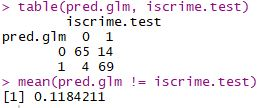
\includegraphics[width=\linewidth, height= 60pt]{Graphics/Assignment1/LogisticRegressionConfusionsMatrix_0001.JPG}
    \caption{Confusion Matrix - sign. level of 0.001}
    \label{fig:logistic_regression_confusions_matrix_0001}
\end{minipage}
\end{figure}


\noindent
\textbf{Linear Discriminant Analysis} \\
In the following experiment with Linear Discriminant Analysis (LDA), the same variables with respect to the significance levels will be used for the model training. Each model has a confusion matrix, which is used to calculate error rate and accuracy. From the models, each variable has a coefficient (Figure \ref{fig:LDA_005_1}, \ref{fig:LDA_001_1} and \ref{fig:LDA_0001_1}), which determine the process growth. The full result of code can be seen on figure \ref{fig:coefficients_method_005}, \ref{fig:coefficients_method_001} and \ref{fig:coefficients_method_0001} in appendix \ref{app:boston_housing}.

Some of the coefficients are negative and some are positive. Negative coefficients indicate the larger the variable the less is the crime rate. The value of said variable determines the influence or the effect on the crime rate. The larger the coefficient the more it affects the crime rate. 

\begin{figure}[H]
\centering
\begin{minipage}{0.32\textwidth}
\centering
    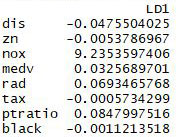
\includegraphics[width=0.8\linewidth]{Graphics/Assignment1/LDACoefficients_005_1.jpg}
    \caption{LDA Coefficients - sign. level 5\%}
    \label{fig:LDA_005_1}
\end{minipage}\hfill
\begin{minipage}{0.32\textwidth}
\centering

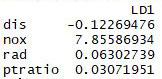
\includegraphics[width=0.8\linewidth]{Graphics/Assignment1/LDACoefficients_001_1.jpg}
    \caption{LDA Coefficients - sign. level 1\%}
    \label{fig:LDA_001_1}
\end{minipage}\hfill
\begin{minipage}{0.32\textwidth}
\centering

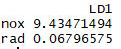
\includegraphics[width=.6\linewidth]{Graphics/Assignment1/LDACoefficients_0001_1.jpg}
    \caption{LDA Coefficients - sign. level 0.1\%}
    \label{fig:LDA_0001_1}
\end{minipage}
\end{figure}

The figures \ref{fig:LDA_005}, \ref{fig:LDA_001} and \ref{fig:LDA_0001} shows the different confusion matrices and error rates for each training of model in respect to their significance level. 

\begin{figure}[H]
\centering
\begin{minipage}{0.32\textwidth}
\centering
    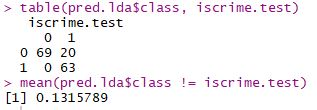
\includegraphics[width=\linewidth, height=50pt]{Graphics/Assignment1/LDAConfusionsMatrix_005.JPG}
    \caption{LDA Confusion Matrix - sign. level 5\%}
    \label{fig:LDA_005}
\end{minipage}\hfill
\begin{minipage}{0.32\textwidth}
\centering

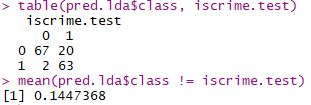
\includegraphics[width=\linewidth, height= 50pt]{Graphics/Assignment1/LDAConfusionsMatrix_001.JPG}
    \caption{LDA Confusion Matrix - sign. level 1\%}
    \label{fig:LDA_001}
\end{minipage}\hfill
\begin{minipage}{0.32\textwidth}
\centering

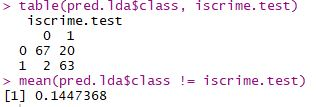
\includegraphics[width=\linewidth, height= 50pt]{Graphics/Assignment1/LDAConfusionsMatrix_0001.JPG}
    \caption{LDA Confusion Matrix - sign. level 0.1\%}
    \label{fig:LDA_0001}
\end{minipage}
\end{figure}



\noindent
\textbf{K-Nearest Neighbors}\\
For this algorithm, the same subsets of variables are used in relation to their significance level. Before the algorithm can be used with the subsets, the data has to be normalized and the optimal \textit{k} values need to be found. In the process of finding the optimal \textit{k's}, a list of \textit{k's} have been evaluated by using the \textit{class} package in R. It enables the use of the method \textit{knn()}. The optimal \textit{k's} will be decided based on their accuracy rates. Figure \ref{app:optimal_ks} in appendix shows a plot with best accuracy and the optimal number of \textit{k's}. The optimal \textit{k's} in the  experiment are 3 and 5. 

\subsubsection*{(c) Description of the findings}
In table \ref{tab:accuracy_and_error_rate_in_relation_to_significance_level} all the results of the algorithms can be seen. According to the results, KNN model has the lowest misclassification rate at $3.9$.  

By choosing KNN results in the highest accuracy. All algorithms performs better than random guessing.


The relevant observed variables is described on table \ref{table_subsets}. The variables are chosen based on the output from logistic regression in figure \ref{fig:task_1_binomial_logistic_model}.

\begin{table}[H]
\centering
\begin{tabular}{|c|c|c|c|}
\hline
Algorithm           & \begin{tabular}[c]{@{}c@{}}Significance \\ Level (\%)\end{tabular} & Accuracy (\%)                                                   & \begin{tabular}[c]{@{}c@{}}Misclassification \\ error rate (\%)\end{tabular} \\ \hline
Logistic Regression & 5                                                                  & 90.14                                                           & 9.86                                                                         \\ \hline
Logistic Regression & 1                                                                  & 87.5                                                            & 12.5                                                                         \\ \hline
Logistic Regression & 0.1                                                                & 88.2                                                            & 11.8                                                                         \\ \hline
LDA                 & 5                                                                  & 86.9                                                            & 13.1                                                                         \\ \hline
LDA                 & 1                                                                  & 85.6                                                            & 14.4                                                                         \\ \hline
LDA                 & 0.1                                                                & 85.6                                                            & 14.4                                                                         \\ \hline
KNN                 & 5                                                                  & \begin{tabular}[c]{@{}c@{}}(k=3) 93.2\\ (k=5) 92.8\end{tabular} & \begin{tabular}[c]{@{}c@{}}(k=3) 6.8\\ (k=5) 7.2\end{tabular}                \\ \hline
KNN                 & 1                                                                  & \begin{tabular}[c]{@{}c@{}}(k=3) 96.1\\ (k=5) 95.4\end{tabular} & \begin{tabular}[c]{@{}c@{}}(k=3) 3.9\\ (k=5) 4.6\end{tabular}                \\ \hline
KNN                 & 0.1                                                                & \begin{tabular}[c]{@{}c@{}}(k=3) 94.8\\ (k=5) 93.4\end{tabular} & \begin{tabular}[c]{@{}c@{}}(k=3) 5.2\\ (k=5) 6.6\end{tabular}                \\ \hline
\end{tabular}
\caption{Accuracy and Error rate in relation to significance level}
\label{tab:accuracy_and_error_rate_in_relation_to_significance_level}
\end{table}

The full r-script is found in appendix listing \ref{lst:Q1_Boston_Housing}.


\subsection{Q-2: Students Performance}

\subsubsection*{(a) Explicit model and probability for scoring an A}

To create an explicit model $L(\textbf{x})$ is calculated using the given $\beta_0$ and $\beta^T$ parameters. The \textbf{x} vector is a variable denoting the time invested in student's study and the student's grade point average. 

\begin{equation*}
    L(\textbf{x}) = \beta_0+\beta^T \textbf{x}=-6+[0.05,1]\begin{bmatrix}x_1 \\ x_2\end{bmatrix}
\end{equation*} 

The result of $L(\textbf{x})$ is put into the logistic regression model to be able to calculate probabilities of a student scoring an A at the exam. $\Pi_1$ will then represent the class of a student scoring an A and \textbf{x} a given student.

\textbf{Logistic Model:}
\begin{equation*}
\mathbb{P}(\Pi_1 | \textbf{x}) = \frac{e^{L(\textbf{x})}}{1+e^{L(\textbf{x})}} = \frac{e^{-6+[0.05,1][x_1, x_2]^T}}{1+e^{-6+[0.05,1][x_1,x_2]^T}}    
\end{equation*}

Given a student who studies 40 hours a week and has a grade point average of 3.5 (C+) the model is used to determine the probability of that student scoring an A at the exam by inserting the given information as $x_1$ and $x_2$.

\begin{equation*}
\mathbb{P}(\Pi_1 | \textbf{x}) =  \frac{e^{-6+[0.05,1][40,3.5]^T}}{1+e^{-6+[0.05,1][40,3.5]^T}} =
\frac{e^{-0.5}}{1+e^{-0.5}} = 0.3775     
\end{equation*}

The student has a 37.8 \% probability of getting an A at the exam.

\subsubsection*{(b) Weeks to study for 80\% chance of scoring an A}

Now the same student from the previous exercise wants to know how many hours of studying each week, that it will take to get a 80\% chance of getting an A to the exam.
To calculate the number of studying hours a week the probability of the logistic model is set to 0.8 and $L(\textbf{x})$ is isolated. Afterwards $x_1$, denoting weakly studying hours, will be isolated in the equation of $L(\textbf{x})$. 

\begin{equation}\label{eq:P}
\mathbb{P}(\Pi_1 | \textbf{x}) = \frac{e^{L(\textbf{x})}}{1+e^{L(\textbf{x})}} = 0.8 \Rightarrow L(\textbf{x}) = 1.386
\end{equation}
\begin{equation}\label{eq:L}
    L(\textbf{x}) = -6+[0.05,1]\begin{bmatrix}x_1 \\ 3.5\end{bmatrix}=1.386 \Rightarrow x_1=\frac{3.886}{0.05}=77.72 hours
\end{equation}

The full mathematical calculations can be seen in Appendix \ref{app:students_performance}.

A student with a grade point average of 3.5 (C+) needs to study 77.72 hours a week to have 80\% chance of scoring an A at the exam.


\section{Alcohol Related Car Crash}
All R code regarding this assignment can be seen in listing \ref{lst:alcohol_related} in appendix \ref{app:alcohol_related_car_crashes}.

\subsection{Identify demographic characteristics}

A binomial logistic model is created of each of the parameters: Gender, Age, Socioeconomic status, with the Accident parameter. We use a binomial logistic model because the dependent variable (Accident) is categorical (Yes/No).
The results were the following:

\begin{itemize}
    \item Accident and Age: Coefficient 1.044 and confidence interval [1.026, 1.064] with p-value $3.14 \cdot 10^{-6}$
    \item Accident and Gender (Male): Coefficient 4.761 and confidence interval [2.348, 10.377] with p-value $3.36 \cdot 10^{-5}$
    \item Accident and Socioeconomic status: 
    \begin{itemize}
        \item Status Middle: Coefficient 1.074 and confidence interval [0.470, 2.416] with p-value $0.864$
        \item Status Upper: Coefficient 1.215 and confidence interval [0.596, 2.502] with p-value $0.592$
    \end{itemize}
\end{itemize}

From these demographics it can be seen that there is a significant association between Age and Accident, and between Gender and Accident given the significance value 0.05.

\subsection{Model}
\textbf{Adjusted:}
First we have to check if the features live up to the three conditions to be a confounder, which are the following: 
\begin{enumerate}
    \item Associated with BAC
    \item Risk factor for Accident (independent of BAC)
    \item Not intermediate factor (BAC is not depended on potential confounder)
\end{enumerate}
The potential confounder: Gender, Age, Socioeconomic status

Condition 2 can already be determined based on the results of the previous exercise. Age and gender both have significant association to Accident, but socioeconomic status has not and will therefore be disregarded.
In relation to condition 1, the association between age and BAC a generalized linear regression is chosen to calculate regression, because both BAC and age are not categorical.
To find association between gender and BAC a binomial model is used, because the dependent variable (gender) is categorical.
The results are the following:

\begin{itemize}
    \item Age: p-value: $2.39 \cdot 10^{-8}$
    \item Gender: p-value: $2.8 \cdot 10^{-4}$
\end{itemize}

It is now shown that condition 1 holds for age and gender since their p-values is under 0.05. 

For condition 3 age and gender are not intermediate factors. If a person drinks a lot, we might be able to tell something about their age or gender, but the fact that a person has a specific age or gender cannot predict anything about their drinking habits. We can now confirm that age and gender are confounders. 

\textbf{Model for adjusted: } 
The adjusted model is when the confounders, age and gender, are included: 

\begin{itemize}

\item The logarithmic coefficient of BAC is 3.78, Gender is 0.92 and Age is 0.022 with the p-value < 0.05

\item The logarithmic confidence interval of BAC is [2.77, 4.97], Gender is [-0.054, 1.93] and Age is [-0.0018, 0.047]

\item The natural coefficient of BAC is 43.76, Gender is 2.51 and Age is 1.02 and confidence interval for BAC is [15.90, 144.08], Gender is [0.95, 6.91] and Age is [1.00, 1.05]

\end{itemize}


\textbf{Model for not Adjusted:}
The unadjusted model is when only looking at BAC and accident. 

\begin{itemize}

\item The logarithmic coefficient of BAC is 4.00 with the p-value < 0.05
\item The logarithmic confidence interval is [3.03, 5.14]
\item The natural coefficient (54.70) and confidence interval [20.77, 171.21]

\end{itemize}

\textbf{Interpret the unadjusted and adjusted odds ratios:}

It is seen that the unadjusted model shows the BAC odds ratio is 54.7. This means that when BAC is increased by 1 the subject has 54.7 times higher odds of getting into an accident. 

The adjusted model shows that BAC odds ratio is 43.7. This means BAC is increased by 1 the subject has 43.7 times higher odds of getting into an accident. 

This shows that when taking age and gender into consideration, there is less chance to get into an accident baed on BAC compared to the unadjusted model. The difference is not that big, so the association does not make a extraordinary difference but it does make a different to some extend.

Since the p-value is $1.2 \cdot 10^{-11}$ of the adjusted model and the p-value is $6.54 \cdot 10^{-14}$ of the unadjusted model, it can be seen that there is a significant association between BAC and car accidents in both models. 


\subsection{Other potential confounder}

Some other potential confounders based on demographics could be the following:
\begin{itemize}
    \item Weight (in kilos)
    \item Vision (Good or Poor)
    \item Medicated (Yes or No)
    
\end{itemize}

A potential confounder could be weight since BAC affects the body more the smaller the weight. A person's weight can be affected by how much they drink, and the weight can maybe have an impact on Accident, but these claims should of course be tested.
For condition 3 intuitively BAC is not depended on weight, because having a specific weight cannot predict their drinking habits.

Vision could also be a factor to look into. The vision might be associated with BAC (condition 1); when drinking alcohol ones vision might get blurred. The vision can be a risk factor for accident independent of BAC (condition 2). Vision is not an intermediate factor(condition 3), because having bad vision not necessarily involve alcohol. 

Finally another potential confounder could be medication. A person drinking alcohol might get worse side effects by being on medication. In that way medication can be associated with BAC. Medication might also be a risk factor for accident to some extend. Also BAC is not dependent on medication, making it an intermediate factor, because taking medication cannot predict their drinking habits.


\subsection{Unadjusted and adjusted models}

The two plots is shown below:

\begin{figure}[!htb]
    \begin{minipage}{.5\textwidth}
        \centering
        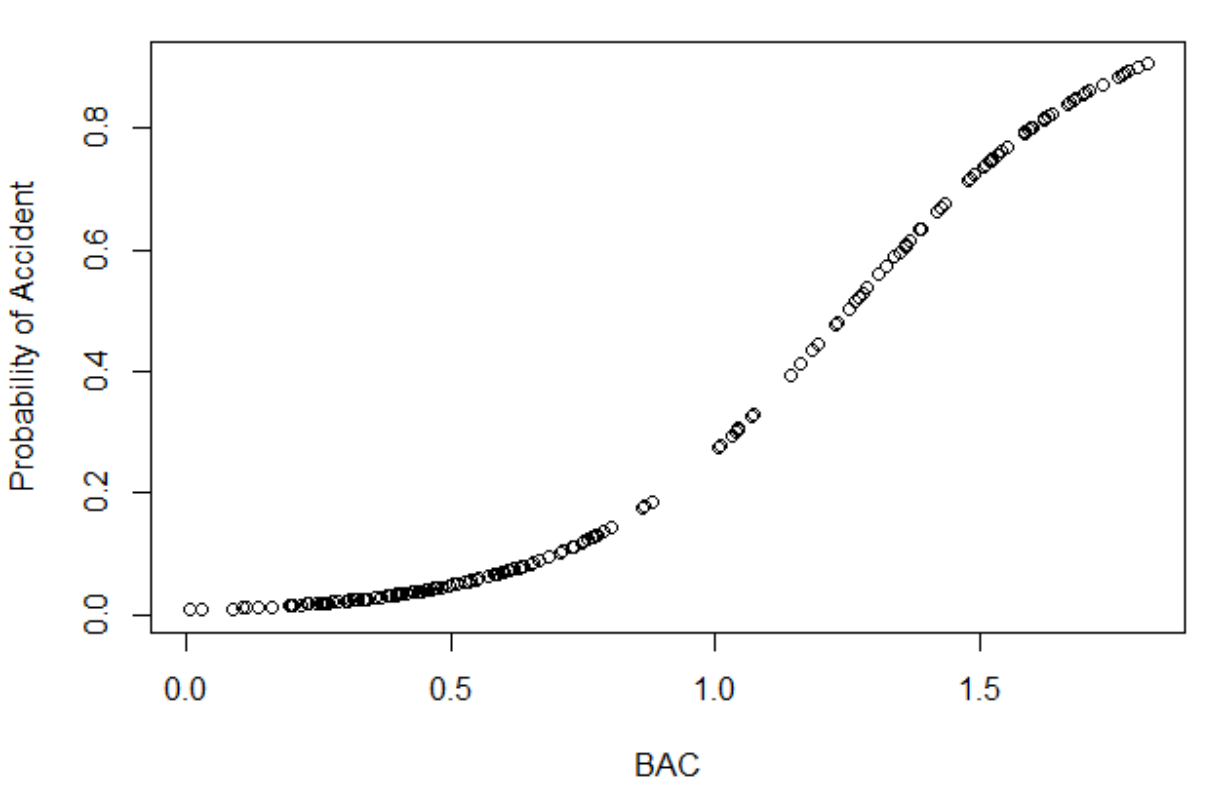
\includegraphics[width=0.9\linewidth]{unadjusted.PNG}
        \caption{Unadjusted Model}
        \label{fig:unadjusted}
    \end{minipage}
    \begin{minipage}{.5\textwidth}
        \centering
        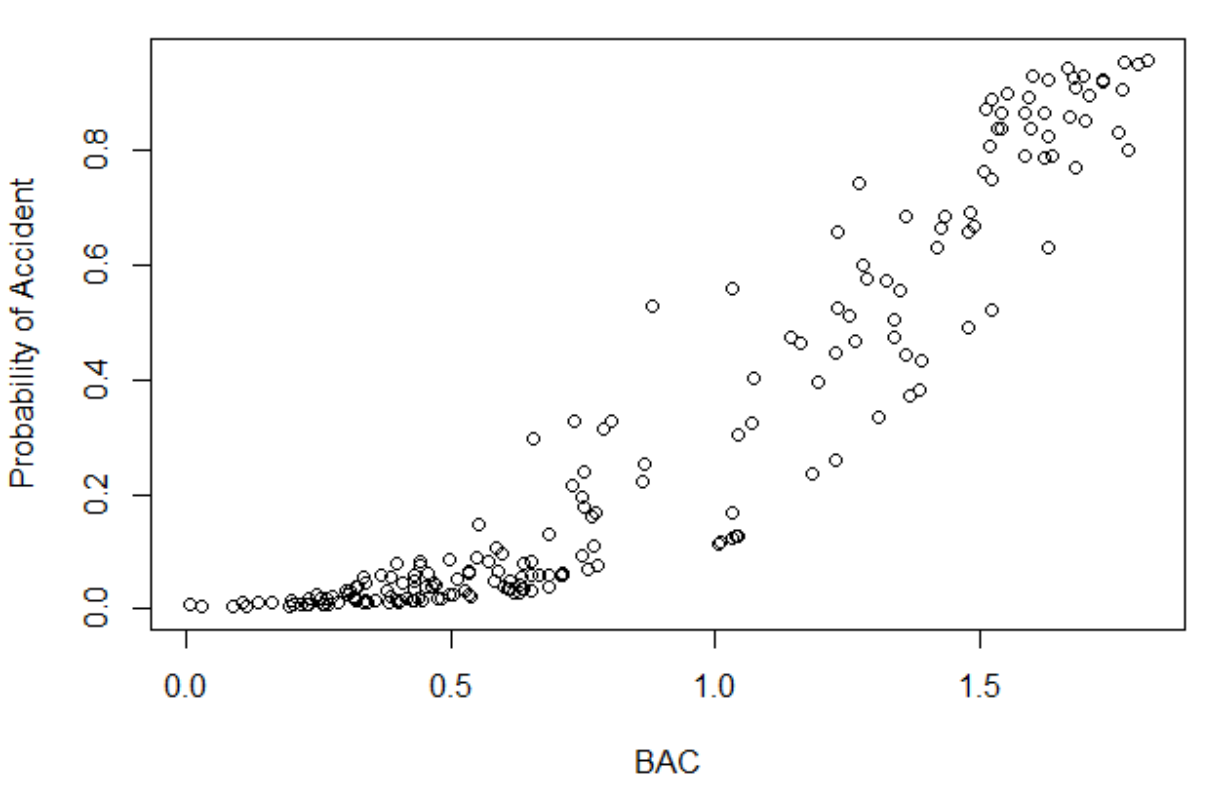
\includegraphics[width=0.9\linewidth]{adjusted.PNG}
        \caption{Adjusted Model}
        \label{fig:adjusted}
    \end{minipage}
\end{figure}

The unadjusted model is fitted directly to BAC as the only independent parameter as seen in figure \ref{fig:unadjusted}. Therefore the points fit a perfect logistic regression as shown in figure \ref{fig:adjusted}.

The adjusted model is fitted to BAC and the two confounders, but since the plot only shows the association of BAC, the points are not fittet as perfectly as the unadjusted model. Now the model is also associated on age and gender, which are disregarded in the plot.

In the adjusted model it can be seen that points are dense approximately below BAC on 0.6 and again it becomes slightly dense when BAC is over 1.5. This can be interpreted as when the BAC is below 0.5 and over 1.5 the model does not rely that much on the confounders, meaning age and gender does not matter when either low or high BAC.

\subsection{Probability}

To calculate the probability of a 40 year old male with BAC > 1, the following equation where used.

$$
\mathbb{P}(BAC > 1) = 1 - \mathbb{P}(BAC \leq 1) = 1 - (\mathbb{P}(BAC = 0) + \mathbb{P}(BAC = 1))
$$

These probabilities were found for 40, 50, 60, 70 and 80 years male with BAC > 1.

\begin{table}[]
    \centering
    \begin{tabular}{|c|c|c|c|c|c|} \hline
        Age & 40 & 50 & 60 & 70 & 80 \\ \hline
        Probability & 0.649 & 0.594 & 0.536 & 0.476 & 0.414 \\ \hline
    \end{tabular}
    \caption{Probability of ages}
    \label{tab:probs_ages}
\end{table}

The differences between the probabilities is plottet in figure \ref{fig:differences_in_ages} in appendix \ref{app:alcohol_related_car_crashes}.

The change is not linear, but it looks as a logistic function.

\subsection{Predictive performance and the threshold value}

After running the model on the new data set a confusion matrix has been produced, comparing the predictive outcome and the observed outcome.

\begin{table}[H]
    \centering
    \begin{tabular}{c|c|c}
      Observed / Predicted & \textbf{Yes} & \textbf{No} \\ \hline
      \textbf{Yes} & 8 & 1 \\
      \textbf{No} & 4 & 4
    \end{tabular}
    \caption{Confusion Matrix}
    \label{tab:my_label}
\end{table}

Using the confusion matrix as seen in table \ref{tab:my_label} different properties are calculated based on figure \ref{fig:confusion_Matrix} Appendix \ref{app:boston_housing}. The following is the calculated values of Accuracy, Precision, Sensitivity and Specificity: 0.71, 0.8, 0.5 and 0.89.

\section{Artist Identification}

%------------------ Start: Chapter intro -----------------
\subsection{Results}
\label{section:Results}
Following sub chapter shows the results and a small explanation. 
% Change the link to where ever the repo will be.

%------------------ End: Chapter intro -----------------

\begin{table}[H]
    \centering
    \begin{tabular}{|l|l|l|l|l|}
        \hline
         & Renoir & Manet & Degas & Monet \\ \hline
        Image 1 & \textbf{9.16161060e-01} & 4.37439530e-06 & 8.38107169e-02 & 2.37891982e-05 \\ \hline
        Image 2 & 6.23026741e-10 & \textbf{8.16067636e-01} & 4.14584717e-03 & 1.79786533e-01 \\ \hline
        Image 3 & 2.28641890e-14 & \textbf{1.00000000e+00} & 1.85917379e-08 & 4.80035141e-08 \\ \hline
        Image 4 & 4.24926483e-10 & 4.80975071e-03 & \textbf{9.95190263e-01} & 1.43515150e-13 \\ \hline
    \end{tabular}
    \caption{Image predictions}
    \label{tab:image_predictions}
\end{table}

All images will be commented from table \ref{tab:image_predictions}.

%------------------ Start: Image 1 -----------------

\subsubsection*{Image 1}

In the first image we can say with a 91.61\% certainty that it is a Renoir painting. Therefore the painting has been classified as drawn by Renoir.
%------------------ End: Image 1 -----------------


%------------------ Start: Image 2 -----------------
\subsubsection*{Image 2}

The second image is with 81.60\% certainty a Manet painting. This is however not true as the painting was painted by Jackson Pollock, but such classification is not available in the output classifier, therefore it picks the next best author, which seems to be Manet in this case. 
%------------------ End: Image 2 -----------------


%------------------ Start: Image 3 -----------------
\subsubsection*{Image 3}

The third image is with 100\% certainty a Manet painting. Therefore the painting has been classified as drawn by Manet.
%------------------ End: Image 3 -----------------



%------------------ Start: Image 4 -----------------
\subsubsection*{Image 4}

The last picture is with 99.51\% certainty a Degas painting. Therefore the painting has been classified as drawn by Degas.


%------------------ End: Image 4 -----------------

The assignment pictures are validated using WikiArt. The correct author can be found in appendix  \ref{app:artist_identification}.  

%------------------ Start: Solution Approach --------------
\subsection{Solution Approach}
The following section describes the process that was committed to get the results for section \ref{section:Results}. Snippets of source code is in the Appendix.\\

\noindent{\textbf{Gather data:}} Data was gathered using a small Bash script [\ref{code:fetch_images}] to quickly download images for a certain artist. This process was repeated for all four artists.\\

\noindent{\textbf{Explore data:}} Gathered data was explored and it was apparent that Manet did not have more than 200 images. This information lead to the decision to use a maximum of 196 images for each artist, excluding the images from the assignment and a couple of images with errors in them. The reason to that was to prevent an artist from being too dominant. An example for a dominant factor would be using 1300 images which Renoir has within the style of impressionism. The 196 images for each artist was put into their own folders, with the artist name as the folder name.\\

\noindent{\textbf{Preparing the data:}} Gathered data was then prepared, for this Python was used. The code [\ref{code:load_data}] iterates through each four folders and process the images one by one. The dimension of the images is set to 224x224 which is a good balance between detailed and size to process. Afterwards the data was shuffled within each artist (not cross shuffle among artists) afterwards split into 80\% training data and 20\% test data [\ref{code:shuffle_and_split_data}]. The training and test data is then used for training and testing the convolutional neural network model.\\

\noindent{\textbf{Picking a pre-trained network:}} To avoid having to create a convolutional neural network from scratch it was decided to make use of an existing neural network. For this VGG16 \cite{DBLP:journals/corr/SimonyanZ14a} has been used that was pre-trained on ImageNet \cite{imagenet_cvpr09}. VGG16 consists of 16 convolutional neural networks.\\

\noindent{\textbf{Transfer Learning with VGG16:}} As mentioned in the previous paragraph an existing model is used. This is to avoid having to train the convolutional neural network from scratch. Therefore transfer learning is made use of [\ref{code:model_creation_and_training}]. This happens in the following steps:
\begin{enumerate}
    \item Adjust image input to 224x224, the same dimension as our images from preprocessing
    \item Load VGG16 model pre-trained on ImageNet [\ref{fig:imagenet_vgg16}]
    \item Take VGG16's block5\_pool layers output.
    \item Feed the block5\_pool output to newly created flatten layer.
    \item Create two fully connected layers with 128 neurons each, using RELU activation as the synapse for deciding if the neuron should fire or not. 
    \item Create an output layer for four classes that makes use of softmax as the classifier
    \item Freeze all the layers except the newly added layers, this is to prevent the weights changing in the remaning layers
    \item Compile the new model which can then be used for training and test. [\ref{fig:custom_vgg16}]
    \item Train the model on the 80\% training data and then evaluate the model on the 20\% test data.
\end{enumerate}

The model is now ready to be used for classification of paintings that are not part of the test and training data. The model has an accuracy of 81.63\% evaluated with the test data. Not exactly the best to classify benign vs malignant tumor, however good enough for art.



%------------------ End: Solution Approach --------------

